% !TEX root = deckblatt2b.tex

\section{Invertierender Verst\"arker}
\subsection{Simulationsschaltung}
\begin{figure}[H]
  \begin{center}
    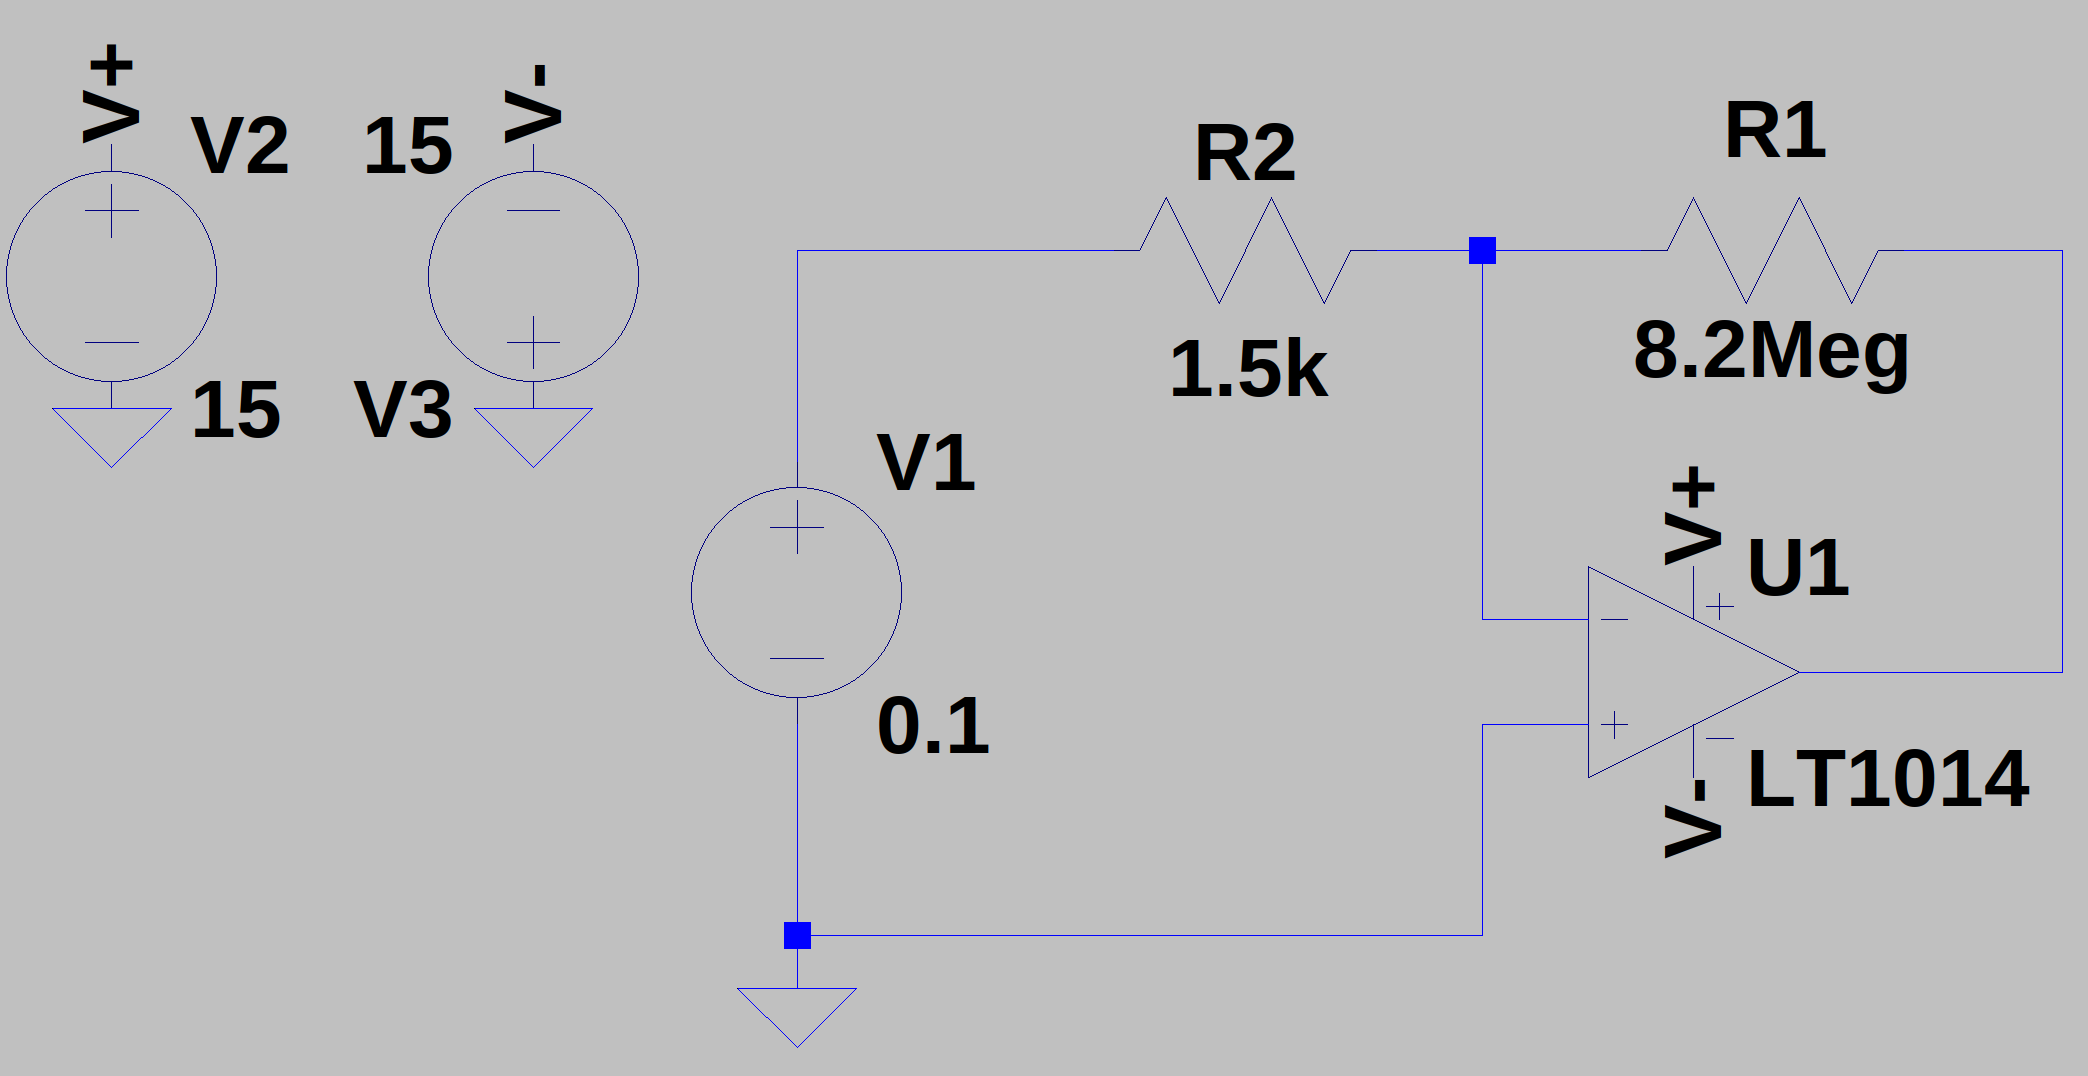
\includegraphics[width=1\textwidth]{./Schaltungen/InvertierenderVerstaerker.png}
    \caption{Simulationsschaltung}
  \end{center}
\end{figure}
\noindent
Da es sich bei dieser Schlatung um einen invertierenden Verst\"arker handel, wird die Eingangsspannung am invertierendne Eingang des OPV geschaltet.
Der Ausgang wird ebenfalls auf den invertierendne Eingang gegengekoppelt umd eine Brauchbare Verst\"arkung einstellen zu k\"onnen. Ein Idealer OPV ohne Gegenkopplung w\"urde die Differenzspannung zwischen invertierenen und nicht-invertierendne Eingang $\infty$ verst\"arken. Die Vert\"arkung wird mit den Beiden Widerst\"anden $R_1$ und $R_2$ eingestellt. Die Beiden Spannungspquellen $V_2$ und $V_3$ stellen die Symetrische Versorgungsspannung von $-15V$ bis $+15V$ dar.\\ \\
$\frac{U_a}{U_e}=\frac{R_1}{R_2} \Rightarrow U_a=U_e*\frac{R_2}{R_1} \Rightarrow V=\frac{R_2}{R_1}$ \\ \\
Da sich die Verst\"arkung $V$ laut Angabe zwichen $-40$ und $-60$ befinden soll wurden f\"ur die Widerst\"ande folgende Werte gew\"ahlt: \\ \\
$R_1=8,2M\Omega$ \\
$R_2=1,5k\Omega$ \\
